\section{不同有效人口下的轨迹分解与临界案例}
\label{app:panel_eta_N}
固定 $\eta=100$ 时的分人口轨迹见图\ref{fig:panel_N_decomp}。

\begin{figure}[htbp]
\centering
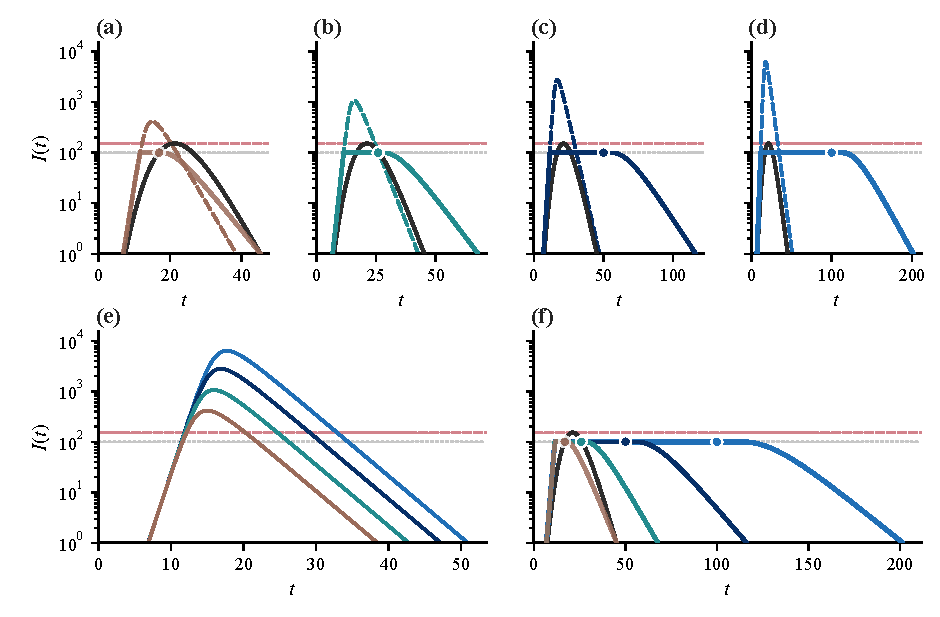
\includegraphics[width=\textwidth]{figures/layout_v5/fig_panel_B_trajectory_decomposition.pdf}
\caption{固定 $\eta=100$ 时不同有效人口下的感染轨迹。(a)--(d) 分别对应 $N_{\rm eff}=3973,10151,26584,60424$，各包含阈值控制、常规控制和固定 TDINN 参照；(e) 比较四个人口规模下的常规控制；(f) 比较阈值控制与 TDINN。横轴 $t$ 的单位为天。}
\label{fig:panel_N_decomp}
\end{figure}
三类临界有效人口下的阈值比较见图\ref{fig:dom:critical-cases}。
\clearpage
\begin{figure}[H]
\centering
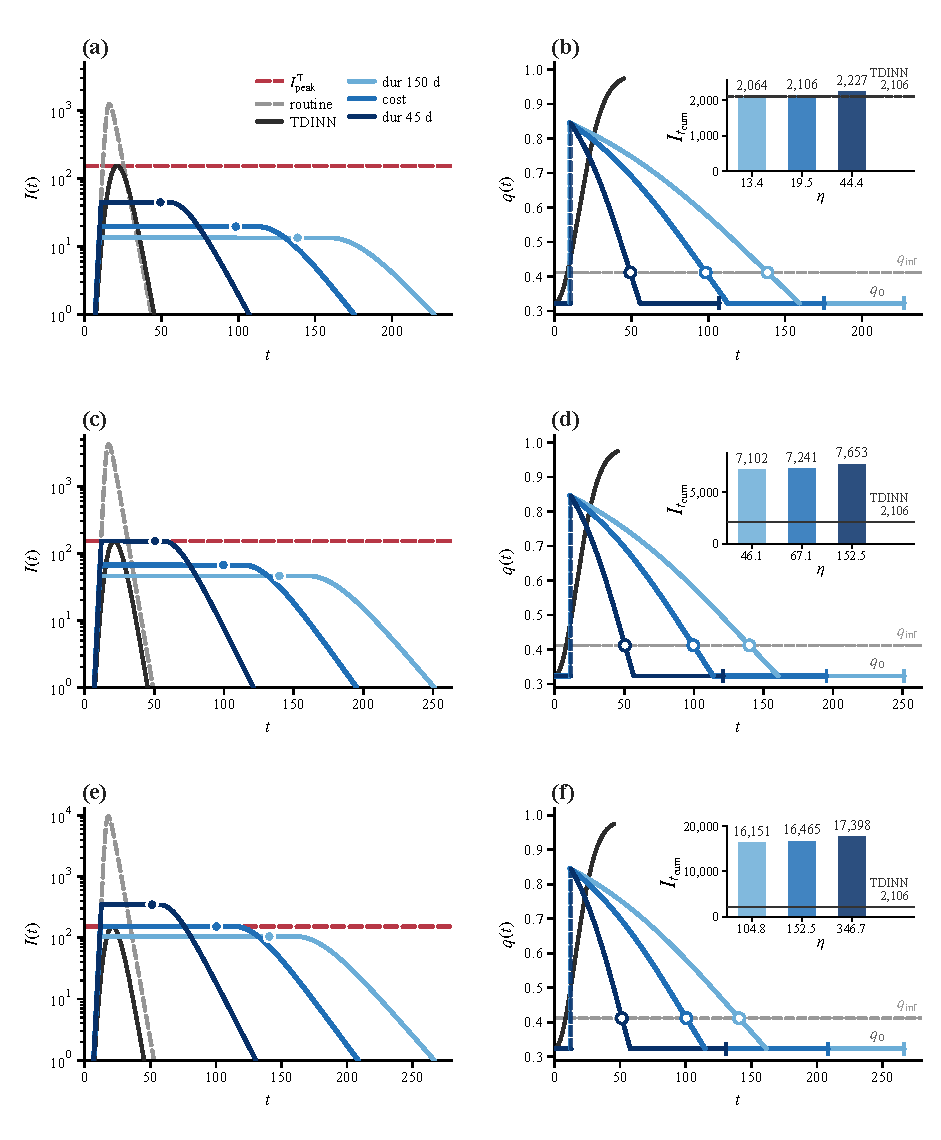
\includegraphics[width=\textwidth]{figures/layout_v5/critical_population_cases.pdf}
\caption{三类临界有效人口下的阈值比较。三行依次为 $N_{\rm eff}=11813,40553,92174$；左列为社区感染者人数（对数纵轴），右列为隔离率，横轴 $t$ 的单位为天。(a) 中的图例适用于三行：蓝色轨迹对应 $150$ d 时长、成本和 $45$ d 时长条件，黑实线为固定 TDINN 参照，灰虚线为同人口常规控制，红虚线为 TDINN 感染峰值。空心圆标记隔离率拐点，水平段上的实心点为该时刻在感染曲线上的投影而非感染曲线的拐点，短竖线为清零时刻。内嵌柱图给出清零时的总累计感染，虚线为 TDINN 参照 $2105.63$。}
\label{fig:dom:critical-cases}
\end{figure}

本附录采用三个阈值比例：
\[
\theta_{\rm dur150}=1.137\times10^{-3},\qquad
\theta_{\rm cost}=1.655\times10^{-3},\qquad
\theta_{\rm dur45}=3.762\times10^{-3}.
\]
初值仍取固定绝对值 $I_0$，不同 $N_{\rm eff}$ 下不重新拟合。三个人口规模分别对应累计感染、45天控制持续时间和成本条件的临界值，结果见图\ref{fig:dom:critical-cases}。各参数组中，拐点相对位置约为 $\lambda=0.861$，绝对时刻随启动时间改变。

当 $N_{\rm eff}=11813$ 时，三个阈值为 $13.432,19.550,44.435$，清零时间分别约为 $227.6,175.5,107.1$ d；成本条件下累计感染约为 TDINN 参照 $2105.63$，另外两个阈值的结果分别低于和高于该参照。当 $N_{\rm eff}=40553$ 时，三个阈值为 $46.113,67.115,152.546$，最后一个约等于 TDINN 峰值。当 $N_{\rm eff}=92174$ 时，三个阈值为 $104.810,152.546,346.725$，分别低于、约等于和高于 TDINN 峰值。



\FloatBarrier
